\documentclass[12pt]{article}

\usepackage{sbc-template}

\usepackage{graphicx,url}

\usepackage[brazil]{babel}   
%\usepackage[latin1]{inputenc}  
\usepackage[utf8]{inputenc}  
% UTF-8 encoding is recommended by ShareLaTex
\usepackage{multirow}

\sloppy

%\title{Instructions for Authors of SBC Conferences\\ Papers and Abstracts}
\title{Criação de um Mecanismo para Encapsulamento e Disponibilização de Funções para Manipulação de Imagens Digitais Usando um Web Service RESTful}
\author{Fernando Henrique Alves\inst{1}, Paulo Henrique Lopes Silva\inst{1}, Leandro Carlos de Souza\inst{1}}
\address{
  Centro de Ciências Exatas e Naturais\\
  Universidade Federal Rural do Semi-Árido (UFERSA) -- Mossoró, RN -- Brazil
  \email{fernandofha01@gmail.com, \{phenrique,leandro.souza\}@ufersa.edu.br}
}

\begin{document} 

\maketitle

%\begin{abstract} 
%\end{abstract}

\begin{resumo} 
  O presente artigo promoveu a criação de um serviço web do estilo arquitetural REST (Representational State Transfer - Transferência de Estado Representacional), proposto por Roy Thomas Fielding, em sua tese de doutorado no ano 2000, com objetivo de disponibilizar funcionalidades de uma API(Application Programming Interface - Interface de Programação de Aplicativos) de PDI(Processamento Digital de Imagens).
  O trabalho se fundamentou em pesquisas bibliográficas, buscando inicialmente construir uma base conceitual bibliográfica, para então implementar uma aplicação de serviços web.
  Cumpridas todas as etapas a que se propôs, o estudo resultou na confirmação da eficácia e viabilidade da adoção de REST no provimento de serviços em um universo de sistemas distribuídos. O grau de dificuldade para implementação foi considerado baixo em termos práticos, mas demandando a necessidade de domínio dos conceitos teóricos envolvidos.
  
  \textbf{Palavras-chave:} Web Service, Interoperabilidade e Processamento Digital de Imagens.
\end{resumo}


\section{Introdução}

Com a evolução da tecnologia, foram desenvolvidas várias facilidades para o ser humano. 
Dentre elas, a Computação e a Internet se destacam por automatizar tarefas, reduzir
custos, distância e tempo para realizar a troca de vários tipos de informação. 

Toda área, seja ela educação, comércio, medicina ou militar, exige troca de informação para seu funcionamento. 
Um dos mais populares modos de comunicação de dados via internet é através do uso de um Web Service(WS) ou serviço web.
Segundo o \cite{w3c1} um WS é definido como um sistema de software projetado para fornecer suporte à interoperabilidade entre máquinas sobre rede.
%Web Services podem ser definidos como aplicações cliente/servidor que se utilizam da comunicação 
%através da internet, por meio do protocolo HTTP (HyperText Transfer Protocol), para prover serviços 
%entre softwares que estejam executando em diferentes plataformas. Essas aplicações podem fazer uso do padrão 
%XML (eXtensible Markup Language) para prover descritores que são interpretados automaticamente 
%por outros sistemas, permitindo assim que diversos programas simples possam interagir uns com os 
%outros para, em conjunto, fornecer soluções mais complexas e sofisticadas.
De acordo com  \cite{cerami:02} este tipo
de serviço permite a comunicação entre aplicações por meio de uma interface bem
definida.

Nos últimos anos, têm-se acompanhado a disponibilização de um grande número de sistemas 
computacionais com um considerável conjunto de recursos que satisfaçam as necessidades de 
desenvolvedores de software. Esse aumento do poder computacional gera um desejo de tratar 
problemas de maior escopo por parte de programadores e pesquisadores, e uma das áreas que podem 
se beneficiar de tal avanço é a de Processamento Digital de Imagens (PDI), pois a popularização 
de dispositivos de aquisição e armazenamento de mídias digitais, como imagens e vídeos, faz 
crescer a demanda por software capaz de manipulá-las.

O PDI refere-se ao processamento de imagens por meio de um computador digital. Segundo \cite{spring} o objetivo de se usar processamento digital de imagens é melhorar o aspecto visual de certas feições estruturais para o analista humano e fornecer outros subsídios para a sua interpretação, inclusive gerando produtos que possam ser posteriormente submetidos a outros processamentos. 

Neste contexto, APIs(Application Programming Interface) podem incorporar implementações de métodos que são a base comum para a manipulação de imagens e 
vídeos a fim de minimizar erros de codificação, diminuir o custo e o tempo de produção. 

De acordo com \cite{pressman:16, sommerville:11} APIs contém a implementação de funcionalidades de uso frequente e que podem ser utilizadas pelo
programador sem que que seja necessário que ele tenha um conhecimento aprofundado sobre a área ou os métodos utilizados.

Com a disseminação da internet e da consequente e inevitável necessidade de troca de informação, 
as aplicações e sistemas desenvolvidos hoje em dia precisam 
atender a certas condições do cenário atual, essas condições dizem respeito às características 
de execução dos softwares de forma distribuída, rápida e portável. 

Diante da necessidade de permitir que uma API de PDI atenda a tais requisitos, surge a
possibilidade de implementar uma ferramenta, independente de plataforma, para a
disponibilização de suas funcionalidades.

Para chegar à ferramenta, a solução está implementada em Linguagem
Java, com auxílio de uma ferramenta denominada Jersey, baseada na arquitetura
SOA(Service-Oriented Architecture), mais especificamente em Serviço Web seguindo o conceito REST, do inglês
Representational State Transfer (Transferência do Estado Representacional). 

De acordo com \cite{oracle} Java é uma linguagem de programação e plataforma computacional cujo lançamento foi realizado pela Sun Microsystems em 1995.

Em \cite{soa1,soa2} temos que SOA é um estilo de arquitetura de software cujo princípio fundamental é o de que as funcionalidades implementadas pelas aplicações devam ser disponibilizadas na forma de serviços.

Proposto por \cite{rest} REST refere-se a um estilo de arquitetura de software.

De acordo com \cite{jersey} Jersey é uma biblioteca de programação que implementa especificações de criação de WSs do tipo REST, baseada na linguagem Java.

Este tipo de Serviço Web utiliza-se do protocolo HTTP(Hypertext Transfer Protocol) para realizar a troca
de mensagens entre clientes e servidor. Outra característica importante é a forma de
redirecionamento de serviços, realizado através de um endereçamento URI(Uniform Resource Identifier)
específico.

Aliando todos os fatores e tecnologias apresentados anteriormente, torna-se
possível o desenvolvimento de um mecanismo baseado em Serviços Web, que disponibilize serviços de uma API de processamento digital de imagens
com baixos custos computacionais, ou seja, baixo consumo de memória e processamento.

\section{Referencial Teórico} \label{sec:firstpage}

Esta seção tem como objetivos desenvolver ideias com base em referências bibliográficas, visando o embasamento teórico do estudo e elucidar quais são os teóricos que já estudaram sobre os assuntos abordados neste trabalho.
% e que lhe ajudarão asustentar, embasar o tema que será desenvolvido.

\subsection{Middleware}

Para \cite{coulouris:05} o middleware refere-se a uma camada de software
que promove uma abstração da programação, assim como o mascaramento de
heterogeneidade das redes, do hardware, de sistemas operacionais e linguagens de
programação subjacentes. Tal camada configura funções de identificação, autorização,
autenticação, segurança, entre outras. O middleware implementa a comunicação e o
compartilhamento de recursos e aplicativos distribuídos.
De acordo com \cite{tanenbaum:07}, um middleware forma uma camada entre aplicações e plataformas distribuídas
cuja finalidade é proporcionar um grau de transparência de distribuição. 
Neste trabalho pretende-se fazer middleware de modo que sejam simples as
configurações, adaptações e personalizações da aplicação conforme sejam necessárias.

\subsection{Web Service}

Com o surgimento da comunicação através das redes de computadores e da necessidade
de diferentes softwares trocarem informações, surgiu o conceito de Webservice (WS).
Os Webservices permitem que sistemas desenvolvidos em diferentes linguagens,
sendo executados em diversas plataformas, transmitam e recebam informações
padronizadas entre si, permitindo uma interação entre os dispositivos, mais abrangente
que qualquer outra tecnologia de computação distribuída existente.

Segundo \cite{kalin:09}, Webservice é um tipo de aplicação para web distribuída,
cujos componentes podem ser aplicados e executados em dispositivos distintos.
Configura-se como um mecanismo de comunicação que permite a interoperabilidade
entre sistemas. 

Para \cite{kreger:01}, um Webservice descreve uma coleção de operações
que são acessíveis pela rede através de mensagens XML (eXtensible Markup Language)
padronizadas. Porém existe a tecnologia JSON (Javascript Object Notation) que
também possibilita a troca de mensagens de forma mais leve. 

Segundo \cite{sandoval:09}, dentre os
formatos mais utilizados nas requisições e respostas, destacam-se texto plano
HTML, XML e JSON. O uso de Webservice
possibilita que aplicações desenvolvidas em plataformas e linguagens diversificadas
troquem informações padronizadas permitindo a interação entre elas com rapidez,
facilidade e baixo custo, conforme ilustrado na Figura 1.

\begin{figure}[ht]
	\centering
	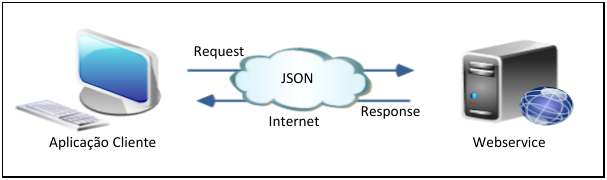
\includegraphics[width=.8\textwidth]{figura1.png}
	\caption{Troca de informações entre uma aplicação cliente e um WebService}
	\label{fig:exampleFigura1}
\end{figure}

\cite{souza04} explica que os Webservices utilizam tecnologias que permitem que
os serviços sejam disponibilizados pela WEB transportando e transformando dados
entre aplicações com base em XML ou JSON. Nesse contexto, o XML e JSON além de
funcionarem como padrão para troca de mensagens também têm o papel de definir os
serviços. Sua sintaxe especifica como os dados são representados, transmitidos e
detalhes de como são publicados e descobertos.

Existem basicamente, dois grupos de serviços web: os serviços baseados em SOAP (Simple Object Access Protocol) e os REST (Representational
State Transfer ). Um serviço baseado em SOAP entregue sobre HTTP é um caso especial dos serviços REST. O foco deste trabalho está na criação e utilização de um web service do grupo REST, devido a sua popularização, e ferramentas auxiliares disponíveis para uso.

\subsubsection{REST - Representational State Transfer}

Descrito por \cite{rest}, REST é um modelo de arquitetura de software distribuído, baseado em comunicação via rede.
%Um sistema no estilo REST é denominado RESTful e possui as seguintes características:
Segundo \cite{richard:07} Um sistema baseado no modelo REST denomina-se RESTful. Para a implementação de tal sistema não há a necessidade da criação de novos protocolos ou tecnologias, pois o mesmo é suportado em qualquer arquitetura de rede.

Enquanto o SOAP é um protocolo de mensagens, o REST é um estilo de arquitetura
de software para sistemas hipermídia distribuídos, conhecidos como recursos e são acessados via URIs (Uniform Resource Identifiers ou, em português, Identificador Uniforme de Recursos). 

Segundo \cite{lecheta:15}, um dos motivos pelos quais o SOAP começou a perder espaço para web services RESTful, foi principalmente, por causa da grande utilização de dispositivos móveis atualmente, que possuem recursos mais escassos, e necessitam de uma forma mais leve para tráfego de dados, pois um WS RESTful, possui uma sintaxe mais elegante e pode transmitir informações utilizando formatos mais leves.

Um recurso RESTful é qualquer coisa que possua um endereço através da web, como por exemplo uma imagem jpg, dados de uma empresa, entre outros, ou seja, sistemas em que as hipermídias são armazenadas em uma rede e interconectadas através de hiperlinks podendo ser acessados e transferidos entre clientes e servidores.

O núcleo da abordagem REST consiste na utilização dos métodos HTTP, que correspondem às operações CRUD (Create, Read, Update, Delete). Cada requisição HTTP inclui um dos métodos apresentados na tabela 1 para indicar qual a operação CRUD que deve ser realizada sobre o recurso.
\begin{table}[ht]
	\centering
	\caption{Métodos HTTP e operações CRUD}
	\label{tab:Table1}
	\smallskip
	\begin{tabular}{ |l|l| }
		\hline
		POST & Cria um novo recurso a partir dos dados requisitados \\ \hline
		GET & Lê um recurso \\ \hline
		PUT & Atualiza um recurso a partir dos dados requisitados \\ \hline
		DELETE & Remove um recurso \\
		\hline
	\end{tabular}
\end{table}

Em termos gerais, um cliente RESTful emite um pedido que envolve um recurso, como
por exemplo, um pedido de alteração. Se este pedido for bem sucedido, uma representação
do recurso é transferido do servidor que hospeda o recurso para o cliente que emitiu o
pedido.


\subsection{Processamento Digital de Imagens(PDI)}

Uma imagem pode ser definida por uma função bidimensional f (x,y) em que x e y são um par de coordenadas espaciais e o valor de f representa a intensidade da
imagem naquele ponto. Quando x, y e os valores das intensidades de f são todos finitos e em quantidades discretas, pode-se dizer que a imagem é uma imagem
digital. Os elementos constituintes das imagens são denominados pixels. O PDI refere-se à utilização de métodos que manipulam imagens digitais e que geram
como resultado outras imagens digitais. De acordo com \cite{gonzalez:08} esta manipulação envolve a utilização dos pixels da imagem de entrada para a geração de novos pixels que formam a
nova imagem de obtida.

Na maioria dos casos, os métodos que se deseja implementar para a manipulação das imagens são mapeamentos, considerando a utilização de uma matemática
básica ou avançada, que utilizam as posições e os valores dos próprios pixels. Entretanto, quando os programadores se deparam com o desenvolvimento de
programas que processam imagens, eles devem se preocupar com outras tarefas que não são estão ligadas à essência do PDI. Exemplos destas tarefas são dados
pela escolha e utilização de APIs para a leitura e gravação de arquivos, criação de interface gráfica ou aplicação de testes para verificação do que foi
implementado. Segundo \cite{gonzalez:08,jain:89} estas nuâncias de implementação podem ser abstraídas através do uso de uma API específica que faça a abstração destas tarefas.

\subsection{API em Desenvolvimento}

API do Inglês Application Programming Interface(ou Interface de Programação de Aplicativos), é um conjunto de rotinas e padrões que são seguidos com o intuito de utilizar a funcionalidade de algum software, onde não há a necessidade de o usuário se ater aos detalhes internos de funcionamento do mesmo, ou seja, sua implementação não necessita ser compreendida pelo usuário. 
Paralelamente a este trabalho, está em processo de desenvolvimento, uma API, livre e de código aberto, que poderá ser utilizada para o desenvolvimento de software na área de PDI, para a manipulação de imagens utilizando-se de técnicas de processamento paralelo, podendo ajudar a diminuir custos e tempo para a produção de programas. Além disso, mais programadores podem utilizá-la para o PDI sem que seja necessário que eles se tornem especialistas na área.
Até o presente momento, foram desenvolvidos dois filtros para aplicação em imagens, sendo eles o filtro preto e branco YIQ, e o filtro de recuperação do canal verde da imagem. Este trabalho tem como foco, a disponibilização das funcionalidades dessa API exposta em específico, que, como já mencionado, está em constante desenvolvimento e mais funcionalidades podem ser adicionadas ao serviço remoto.

\section{Desenvolvimento}

Esta seção está destinada a descrever a arquitetura e funcionamento da ferramenta proposta, bem como a disponibilização de seus serviços, e as tecnologias envolvidas em sua implementação.


%A função de um middleware é tornar possível a comunicação entre aplicações que
%não se comunicam diretamente. Para o contexto deste trabalho, que é o de promover a disponibilização das funcionalidades de uma API de PDI, o uso de um middleware é de fundamental
%importância, pois torna possível para que programadores, o torna flexível para novas possibilidades de comunicação com outras
%funcionalidades dos AVA, além da possibilidade de registrar o log de transações
%realizadas entre as partes e outras questões relacionadas à segurança. O middleware foi 
%desenvolvido baseado num padrão de interoperabilidade que permite a comunicação
%com diversos AVA. 

A Figura 2 representa o diagrama da estratégia de comunicação que
foi desenvolvida em duas etapas: entre a aplicação cliente e o WS via HTTP utilizando JSON como padrão de comunicação e entre
o WS e a API de PDI desenvolvida via linha de comando, esta, que por sua vez, está localizada no mesmo servidor do web service.

Para a troca de informações adotou-se o JSON (JavaScript Object Notation). O
JSON é um formato de interconexão de dados utilizado em ambientes cliente-servidor
que possibilita o desenvolvimento nas mais variadas linguagens. O JSON atualmente
vem sendo utilizado como linguagem padrão para comunicação entre sistemas nas mais
diversas plataformas. A disponibilidade de APIs que realizam processamento desse objeto de comunicação e o desempenho proporcionado
pela simplicidade da transmissão de dados utilizando JSON influenciaram na decisão
por utilizá-lo.

A interoperabilidade entre a aplicação cliente e a API de PDI, conforme ilustrado na Figura 2, é
realizado da seguinte forma:
\begin{itemize}
	\item A aplicação cliente se conecta ao web service através da URL de acesso a algum serviço disponibilizado pelo mesmo, informando junto com a requisição, a imagem alvo a qual se deseja realizar tal transformação, codificada no formato base64;
	\item O WS recebe a requisição, decodifica a imagem requisitada, salva-a no disco, e realiza uma chamada via linha de comando para o sistema operacional do servidor, passando como parâmetro o caminho da imagem salva, e o tipo de transformação que se deseja realizar na mesma, para que a API possa realizar seu trabalho;
	\item Após realizar seu processamento, a API retorna para o WS como resultado de execução, a imagem transformada e codificada no formato base64;
	\item O WS por fim, retorna para a aplicação cliente do serviço, um código de status da requisição, representando o sucesso ou insucesso da operação, em conjunto com uma mensagem informando se houve qualquer erro em algum dos passos anteriores, e caso todo o processo tenha sido realizado com sucesso, retorna também a imagem processada pela API, também no formato base64.
\end{itemize}

\begin{figure}[ht]
	\centering
	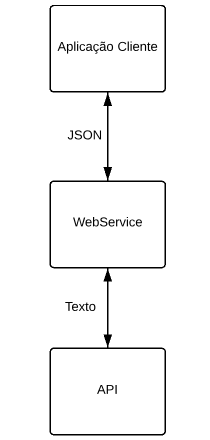
\includegraphics[width=.3\textwidth]{modelo-comunicacao2.png}
	\caption{Modelo de Comunicação}
	\label{fig:Figura2}
\end{figure}

Para que o processo funcione adequadamente, a API precisa estar ao alcance do web service, ou seja, localizada no mesmo servidor, e também é necessário que a mesma implemente a forma padronizada de comunicação descrita anteriormente: enviar como resposta à suas chamadas de funções, uma imagem codificada no formato base64, para que o
WS consiga se conectar à mesma e, dessa forma, interagir com as aplicações clientes conforme o esperado.

O WS será executado em um servidor de aplicação. Este servidor
é responsável por estabelecer a comunicação com as aplicações clientes que desejem utilizar os serviços da API. 
A desvantagem é que recursos computacionais de um servidor serão alocados para o WS, porém, como vantagens teremos a flexibilidade, melhoria no desempenho, manutenibilidade e disponibilidade do serviço.

A utilização das funcionalidades da API de forma direta, necessitando de tê-la instalada na própria máquina do utilizador, traria alguns inconvenientes, sendo eles:
\begin{itemize}
	\item O usuário necessitar instalar novas versões da mesma à medida que novas funcionalidades forem sendo adicionadas;
	\item Dependência de plataforma, uma vez que para se comunicar corretamente com a API, o usuário necessita utilizar a mesma linguagem de programação com a qual a mesma fora implementada;
	\item Restrição de utilização da API à medida que os recursos da máquina do usuário foram ficando mais escassos, uma vez que todo o processamento da API será feito no computador do usuário.
\end{itemize}
%O uso do MiddleWare desonera o consumo da bateria e o processamento do aparelho que esteja executando o mesmo, ampliando sua performance.

O WS possui a implementação e uso de dois serviços através dos quais será possível realizar diversas operações de troca de informações, à medida que novas funcionalidades forem sendo disponibilizadas pela API, poderão ser adicionados novos serviços que correspondam às mesmas.
Todos os serviços possuem somente um parâmetro de entrada (Requisicao) e um parâmetro de saída (Resposta) de tipos que encapsulam as informações necessárias para realizar as requisições e o resultado da operação. Os serviços são descritos a seguir:

%\textit{ListFilters}: Operação destinada a realizar consultas dos filtros disponíveis para aplicação;

\textit{GreenFilter}: Operação destinada a realizar a aplicação do filtro de cor verde na imagem requisitada;

\textit{BlackAndWhiteFilter}: Operação destinada a realizar a aplicação do filtro de cores preto e branco na imagem requisitada.

A definição dos elementos de comunicação – ou objetos de comunicação – é
determinante para o sucesso de todo o processo de comunicação, que inicia na requisição da aplicação cliente, passa pelo WS, chega na API, e finaliza na resposta final do web service. Esses objetos são as estruturas de dados que carregam as informações necessárias para consumir e responder um WS.
A dinâmica de comunicação é realizada da seguinte forma: a aplicação cliente realiza uma requisição encapsulando um objeto de comunicação que é processado pelo web service. Em seguida, o WS realiza uma chamada à função requisitada pelo cliente à API, esta que por sua vez, realiza seu processamento, e envia uma resposta ao WS, que, por fim, responde à requisição do cliente através de um outro objeto de comunicação.

Por exemplo: para consumir o serviço GreenFilter a aplicação cliente requisita através do objeto de comunicação Requisicao os dados da imagem codificada. Em seguida, o serviço GreenFilter envia a resposta com o objeto de comunicação Resposta.

A tabela 2 representa um exemplo da estrutura de dados de um objeto de
comunicação exemplificado no formato JSON.

\begin{table}[ht]
	\centering
	\caption{Descrição dos atributos de comunicação}
	\label{tab:Table2}
	\smallskip
	\begin{tabular}{ |l|l|l| }
		\hline
		Objeto de Comunicação & Atributos & Exemplo (JSON) \\ \hline
		Requisicao & Img: texto & \{“img" : “/9j/4AAQSkZJRgABAQAAAQAB"\} \\ \hline
		\multirow{3}{*}{Resposta} & Status: inteiro & \{“Status": 1, \\
		& Msg: texto & “Msg":“Sucesso", \\
		& Img: texto & “Img":“/9j/4AAQSkZJRgABAQAAAQAB"\} \\
		\hline
	\end{tabular}
\end{table}

A Figura 3 representa o diagrama de sequência para o consumo do serviço GreenFilter:

\begin{figure}[ht]
	\centering
	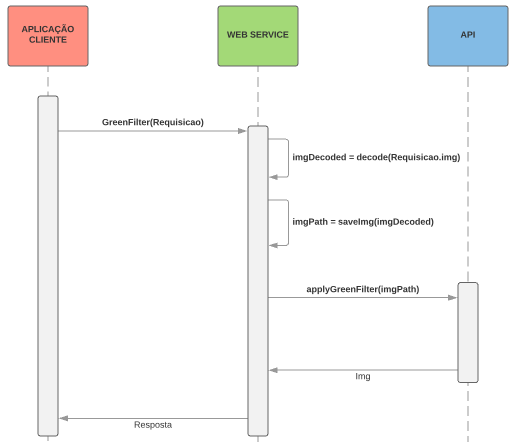
\includegraphics[width=.7\textwidth]{ds-green-filter2.png}
	\caption{Diagrama de Sequência - GreenFilterService}
	\label{fig:Figura3}
\end{figure}

\subsection{Tecnologias Envolvidas}

Nesta seção, serão descritas, bem como o título da mesma explicita, as tecnologias envolvidas na criação deste trabalho, sendo elas, a especificação Java EE; a ferramenta de automatização de construção e gerenciamento de projetos Java, Apache Maven; o framework Jersey, que implementa todas as características da arquitetura REST, ou seja, que nos permite a criação de sistemas RESTful, e por fim, as tecnologias que nos permite o armazenamento e transmissão de informação no formato de texto: JSON e base64.

\subsubsection{Java Enterprise Edition(Java EE)}

Como mencionado na introdução deste trabalho, a linguagem escolhida para desenvolvimento do WS foi Java, que é uma das linguagens de desenvolvimento multiplataforma mais conhecidas e atualmente está bastante consolidada no mercado, com vários fóruns e comunidades dispostos a nos auxiliar no processo de construção de software, o que torna tal escolha bastante razoável. 

O Java EE consiste de uma série de especificações bem detalhadas, ditando como deve ser implementado um software capaz de realizar serviços de infraestrutura, como web services, persistência em banco de dados, gerenciamento de conexões HTTP, acesso remoto, gerenciamento de sessão web, entre outros. Tudo isso, claro, baseado na linguagem Java.

\subsubsection{Framework Jersey}

Como o Java EE é apenas uma especificação, fez-se o uso de um dos principais frameworks utilizados para desenvolver aplicações RESTful em Java, o Jersey, que implementa todas as características da arquitetura REST. Para fazer uso da ferramenta, basta adicioná-la como dependência no arquivo pom.xml, assim como no exemplo da Figura \ref{fig:Figura5}. Após a inclusão da dependência, é necessário alterar mais um arquivo xml de configuração denominado web.xml, localizado no diretório src/main/webapp/WEB-INF, como segue na Figura 9:

\begin{figure}[ht]
	\centering
	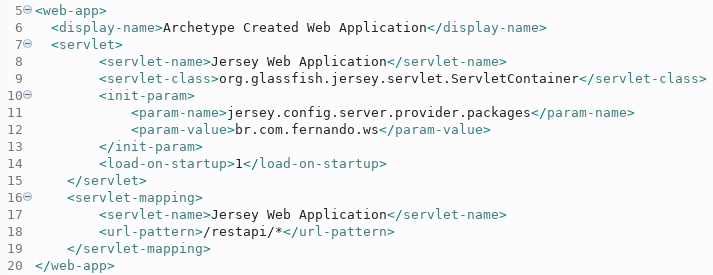
\includegraphics[width=.9\textwidth]{web-xml.png}
	\caption{Arquivo de configuração web.xml}
	\label{fig:Figura9}
\end{figure}

Na Figura acima, a linha 12 refere-se ao pacote java onde estarão salvas as classes referentes aos recursos do web service, já na linha 18, está sendo definida a Url base a qual a partir da mesma será possível o acesso aos recursos, ou seja, no momento, o servidor está sendo acessível pelo seguinte endereço web: \url{http://endereco_ip_servidor:8080/nome_projeto/restapi}.
Em seguida, é necessário a criação de tais classes. Neste trabalho, foi criada a classe MyResource, no pacote descrito pela linha 12 da Figura \ref{fig:Figura9}, A Figura \ref{fig:Figura10} mostra a implementação da classe que expõe os métodos como serviços REST:

\begin{figure}[ht]
	\centering
	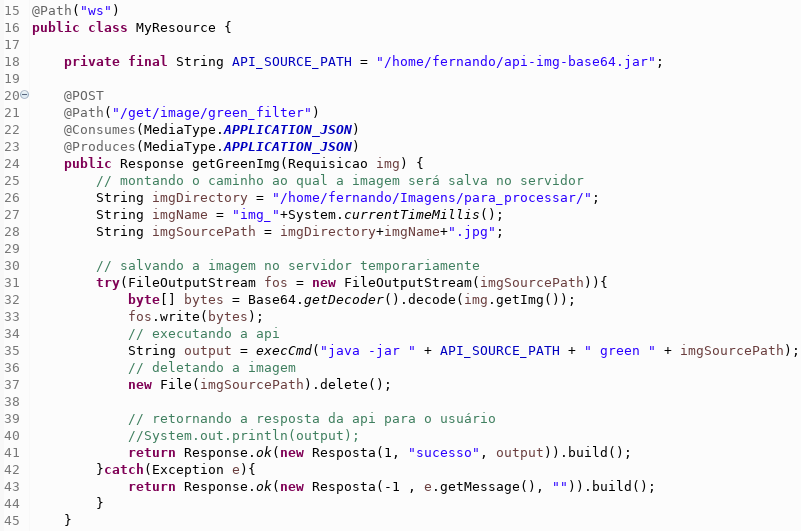
\includegraphics[width=.9\textwidth]{codigo-green-service.png}
	\caption{Classe MyResource - código referente ao serviço greenService}
	\label{fig:Figura10}
\end{figure}

A anotação @Path definida na classe, indica o endereço por meio do qual o recurso será acessado, em conjunto com as anotações @Path, nos métodos implementados pela classe, por exemplo, o método getGreenImg(serviço GreenService), que possui a anotação @Path com o valor /get/image/green\_filter poderá ser acessado por meio da Url \url{http://endereco_ip_servidor:8080/nome_projeto/restapi/ws/get/image/green_filter}.
 O método getGreenImg recebe como parâmetro um objeto do tipo Requisicao, e envia como resposta um objeto do tipo Resposta, ambos descritos na tabela 2. Para acessar esse método, é necessário indicar no cabeçalho da requisição que se deseja acessar o método com tipo de resposta APPLICATION\_JSON. As anotações @POST, @Consumes, e @Produces, dizem respeito ao método/verbo HTTP pelo qual o serviço pode ser acessado, o tipo hipermídia que o serviço aceita como corpo da requisição, e o tipo de hipermídia que o serviço retornará à aplicação cliente, respectivamente. Há também outro método chamado getBlackAndWhiteImg, porém, como o mesmo é muito semelhante ao anterior, decidiu-se omitir sua implementação.

\subsubsection{Armazenamento e transmissão de informação}

Como forma padrão de comunicação entre servidor e cliente, foi adotado o JSON. O JSON é um formato de troca de dados entre sistemas independente de linguagem de programação derivado do JavaScript[1][2]; a Figura \ref{fig:Figura4} exibe um exemplo de arquivo JSON, com a representação de um array de carros, onde cada elemento do array possui os atributos modelo e ano:

\begin{figure}[ht]
	\centering
	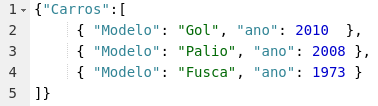
\includegraphics[width=.7\textwidth]{exemplo-json.png}
	\caption{Exemplo de representação JSON}
	\label{fig:Figura4}
\end{figure}

Para que fosse possível a transmissão de um arquivo binário de forma leve e eficiente, foi utilizado o padrão de codificação base64, que nada mais é do que uma forma de representar arquivos binários(imagens, no contexto deste trabalho) em formato de texto, método comumente utilizado na internet para transferência de dados.
Seu nome é dado pelo fato de o mesmo ser constituído por 64 caracteres ([A-Za-z0-9], "/" e "+"). Trabalha com transformação em bits a partir de um outro padrão, como por exemplo ASCII. A tabela 3 expressa um exemplo de codificação da palavra “Fer”.

\begin{table}[ht]
	\centering
	\caption{Exemplo de codificação base64}
	\label{tab:Table3}
	\smallskip
	\begin{tabular}{ |l|l|l|l| }
		\hline
		Conteúdo & F & e & r \\ \hline
		ASCII & 70 & 101 & 114 \\ \hline
		Padrão em Bit & 01000110 & 01100101 & 01110010\\ \hline
	\end{tabular}
\end{table}

Em seguida a cada 6 bits da esquerda para a direita, os valores são convertidos para decimal e posteriormente o algoritmo base 64 entende estes decimais como índices para serem convertidos a um dos 64 caracteres, como mostra o exemplo a seguir:

\begin{table}[ht]
	\centering
	\caption{Exemplo de codificação base64}
	\label{tab:Table4}
	\smallskip
	\begin{tabular}{ |l|l|l| }
		\hline
		Bits & Decimal & Base 64\\ \hline
		0 1 0 0 0 1 & 17 & R \\ \hline
		1 0 0 1 1 0 & 38 & m \\ \hline
		0 1 0 1 0 1 & 21 & V \\ \hline
		1 1 0 0 1 0 & 50 & y \\ \hline
	\end{tabular}
\end{table}

Na tabela 5 confere-se os índices de conversão para base64.

\begin{table}[ht]
	\centering
	\caption{Tabela de índices base64}
	\label{tab:Table5}
	\smallskip
	\begin{tabular}{ |l|l|l|l| }
		\hline
		Value Char&Value Char&Value Char&Value Char \\ \hline
		0	A&	16	Q&	32	g&	48	w \\ \hline
		1	B&	17	R&	33	h&	49	x \\ \hline
		2	C&	18	S&	34	i&	50	y \\ \hline
		3	D&	19	T&	35	j&	51	z \\ \hline
		4	E&	20	U&	36	k&	52	0 \\ \hline
		5	F&	21	V&	37	l&	53	1 \\ \hline
		6	G&	22	W&	38	m&	54	2 \\ \hline
		7	H&	23	X&	39	n&	55	3 \\ \hline
		8	I&	24	Y&	40	o&	56	4 \\ \hline
		9	J&	25	Z&	41	p&	57	5 \\ \hline
		10	K&	26	a&	42	q&	58	6 \\ \hline
		11	L&	27	b&	43	r&	59	7 \\ \hline
		12	M&	28	c&	44	s&	60	8 \\ \hline
		13	N&	29	d&	45	t&	61	9 \\ \hline
		14	O&	30	e&	46	u&	62	+ \\ \hline
		15	P&	31	f&	47	v&	63	/ \\ \hline
	\end{tabular}
\end{table}

\subsubsection{Apache Maven}

Inicialmente, para criação do projeto, utilizou-se da ferramenta de automatização de construção e gerenciamento de projetos Java, denominada Apache Maven, embora também possa ser utilizada com outras linguagens. Ela fornece aos desenvolvedores uma forma padronizada de automação, construção e publicação de suas aplicações.

O processo de criação de um projeto Java EE envolve vários passos, como a criação e organização de seus diretórios, a configuração de diversos arquivos XML, a obtenção de bibliotecas e recursos para o projeto, a geração dos pacotes de publicação, o processo de documentação, entre outras etapas. Normalmente, sem a utilização de tal ferramenta, cada projeto teria sua própria estrutura, seu próprio jeito de gerar pacotes(jar, war), ou de executar cada um desses passos. Projetos complexos, com vários módulos, podem exigir uma ordem específica para a compilação dos mesmos, para que se chegue ao pacote final. Essa não-padronização, pode acarretar vários problemas, como por exemplo, um desenvolvedor alterar a estrutura de pastas do projeto referente a localização de imagens, e esquecer de avisar aos demais, o sistema passaria a funcionar de forma instável em alguns momentos. Tendo em vista esses pontos, e o fato de que tal ferramenta incentiva a adoção de boas práticas, optou-se por utilizá-la.

Após a criação de um projeto Maven, temos à disposição, uma de suas funcionalidades mais poderosas, que é a gestão de dependências, por meio do arquivo pom.xml, que fica localizado no diretório raiz do projeto. Esse arquivo xml nos fornece uma forma fácil de administrar bibliotecas de terceiros necessárias para o funcionamento correto do código, tarefa que pode se tornar difícil, à medida que o projeto for aumentando de proporção e que cada vez mais a adição de bibliotecas ao desenvolvimento se torne necessária. O arquivo pom.xml, além de conter uma lista das chamadas dependências, possui várias outras informações referentes ao correto funcionamento do Maven. Entre outras palavras, ele é basicamente o coração da ferramenta. 
Por meio da lista de dependências, a ferramenta faz uma análise e tenta localizá-las, com o intuito de disponibilizá-las para o projeto. Para realizar as buscas de dependências, o Maven faz uma varredura em locais denominados repositórios, cujos tipos principais são local e público. O primeiro fica localizado na máquina onde a ferramenta está sendo executada(no caso deste trabalho, /home/fernando/.m2/repository/), e o último, em \url{http://repo.maven.apache.org/maven2/}, endereço do repositório público oficial da ferramenta.

A Figura \ref{fig:Figura5} exibe as dependências adicionadas ao arquivo pom.xml deste trabalho, que no caso, são referentes à ferramenta Jersey.
\begin{figure}[ht]
	\centering
	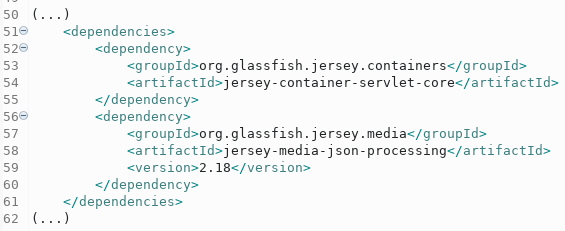
\includegraphics[width=.9\textwidth]{jersey-pom.png}
	\caption{Jersey como dependência Maven}
	\label{fig:Figura5}
\end{figure}

%Outra capacidade da ferramenta é identificar as dependências das dependências do projeto. Ou seja, se uma biblioteca depender de outras, o Maven irá procurar por elas também e assim sucessivamente, até todas as dependências necessárias estarem à disposição do projeto.

Com as dependências citadas na Figura \ref{fig:Figura5} adicionadas, e com o Maven instalado devidamente na máquina, basta um único comando(mvn install), no diretório raiz do projeto, para que a ferramenta realize seu trabalho de baixar dependências que ainda não tenham sido adicionadas ao projeto, compilá-lo e gerar o pacote, com o código compilado.

\section{Estudo de caso}

Nesta seção, serão descritos os passos necessários para a realização de consumo dos serviços da API por meio da comunicação com o WS, apresentando o desenvolvimento de uma aplicação cliente como estudo de caso.

A escolha da linguagem JavaScript como base para o desenvolvimento da aplicação cliente, se deu mais pela necessidade de demonstrar a independência de plataforma que o WS nos proporciona, e também pelo fato de que atualmente JavaScript é uma das linguagens mais conhecidas e utilizadas ao redor do mundo.

A Figura \ref{fig:Figura6} representa a interface da aplicação cliente desenvolvida.

\begin{figure}[ht]
	\centering
	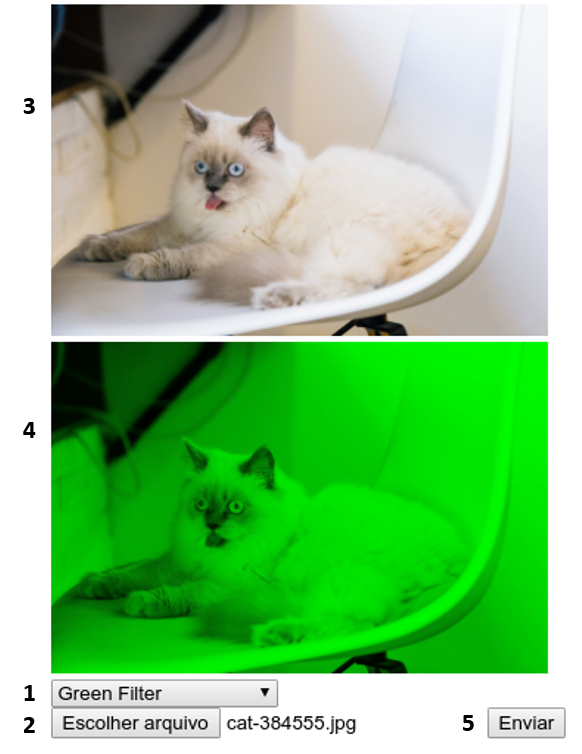
\includegraphics[width=.5\textwidth]{aplicacao-cliente.png}
	\caption{Aplicação Cliente}
	\label{fig:Figura6}
\end{figure}

Esta aplicação consiste em uma página HTML, que utiliza-se da linguagem javascript para realizar as requisições ao Webservice. Na Figura acima, temos a lista de serviços disponibilizados pelo WS(1), onde o usuário poderá escolher qual filtro aplicar, um botão para selecionar a imagem desejada(2), a imagem escolhida(3), a imagem final(4), após o processamento da API, e resposta do middeware, e por fim, o botão de enviar(5), que realizará a requisição.

O código da Figura \ref{fig:Figura7} diz respeito ao código necessário para realizar a requisição aos serviços do webservice:

\begin{figure}[ht]
	\centering
	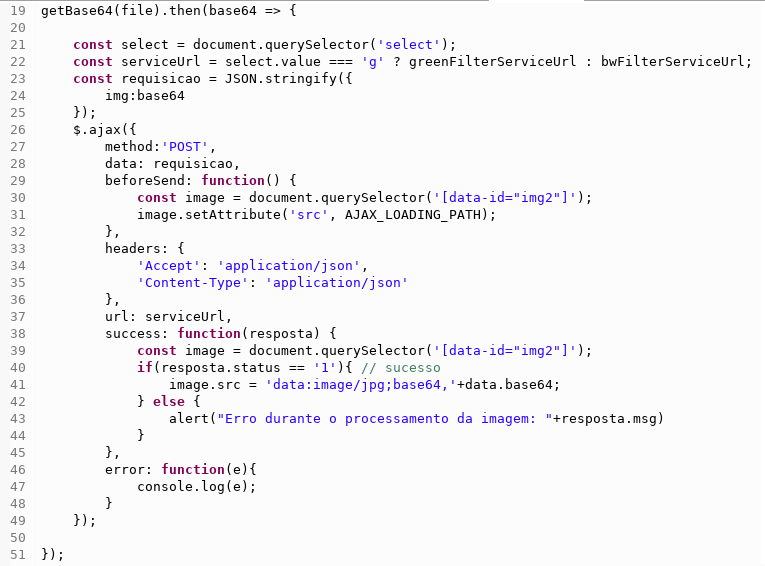
\includegraphics[width=.9\textwidth]{cliente-requisicao.png}
	\caption{Código responsável pela requisição ao webservice}
	\label{fig:Figura7}
\end{figure}

Como a maioria das linguagens de programação possuem suporte à codificação e decodificação do formato base64, por o mesmo ser bastante difundido, não há necessidade de explicar o seu funcionamento. Portanto, no código listado acima, a partir da linha 21, entende-se que a imagem selecionada já está codificada em tal formato, e que seu valor está atribuído na variável denominada "base64". 

Assim sendo, na linha 22, têm-se a definição de qual serviço o usuário escolheu, atribuindo-o à variável serviceUrl, que mais tarde será utilizada para redirecionar a requisição para o serviço correto. A Figura \ref{fig:Figura8} exibe as URLs associadas a cada serviço do webservice. Como o WS está localizado na máquina local, seu acesso se tem por meio da URL \url{http://localhost:8080/demorest/restapi/ws}; 

\begin{figure}[ht]
	\centering
	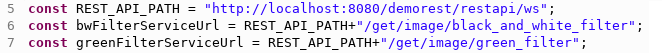
\includegraphics[width=.9\textwidth]{caminho-servicos.png}
	\caption{Urls referentes aos serviços disponibilizados}
	\label{fig:Figura8}
\end{figure}

A linha 23 é responsável pela criação e atribuição de um objeto de comunicação JSON com o atributo Img, como já descrito na tabela 2; 

A partir da linha 26, têm-se de fato a requisição. Com o intuito de simplicidade e praticidade, foi utilizada uma biblioteca javascript chamada jquery, para realização das requisições, e seu uso é demonstrado a partir da linha 26, onde está sendo chamado o método ajax, por meio do objeto \$(cifrão), método este, que nos permite realizar requisições assíncronas, ou seja, o fluxo do código não é interrompido até que a resposta seja obtida. Pelo contrário, após realizar a requisição, a resposta é obtida em um momento posterior, de forma independente, e tratada por meio de uma função (chamada função de callback) que será executada após o término da requisição. Com uma sintaxe bastante simples, esse método nos permite enviar e tratar o resultado de requisições assíncronas:

Linha 27: informamos qual método/verbo HTTP será utilizado na requisição;

Linhas 33 a 36: informamos ao WS, sob qual formato os dados do corpo da requisição foram encapsulados, e sob qual formato a aplicação cliente espera receber como resposta à sua requisição;

Linha 37: informamos a URL para a qual enviaremos a requisição;

Linha 28: enviamos alguma informação no corpo da requisição;

Linhas 29 a 32: o argumento beforeSend recebe uma função que é executada antes de a requisição ser enviada. Nesse caso, atribuímos um "gif" no local onde será inserido a imagem processada pela API, para demonstrar ao usuário que o processo de requisição ainda não foi concluído;

Linhas 38 a 45: a função de callback success é executada quando a requisição é finalizada com sucesso, e nos permite tratar o retorno do servidor, que é recebido por meio do parâmetro "resposta";

Linhas 46 a 48: a função de callback error, por sua vez, é executada quando ocorre algum erro na requisição. De modo semelhante, a mensagem de erro é recebida no parâmetro "e".
%recebe como parâmetro, um objeto javascript, que servirá como base para configurar o funcionamento da requisição:

\section{Considerações Finais}

O principal objetivo do WS desenvolvido é possibilitar aos desenvolvedores uma forma fácil e intuitiva de utilizar as funcionalidades da API apresentada na seção 2.4 por meio de requisições HTTP. Para isso, o programador não deverá encontrar dificuldades em adaptar a sua forma de desenvolvimento atual para um arquitetura de comunicação distribuída.

\bibliographystyle{sbc}
\bibliography{sbc-template}

\end{document}
